The executed finite grid has sixty configuration records and 4,320 candidate evaluations. Its zero-saving reference selects conventional delivery for P2 and P3 at the arbitrary diagnostic price of \$300 each with refundable escrow. Supplied scenario weights yield \$193.50 expected contribution, \$300 successful contribution, a \$40 worst named loss and \$230 required opening cash, including a \$50 reserve. These numbers are accounting-test conditions, not an S3 forecast. The new instrument is not selected in that reference. All sixty records permit an unrestricted conventional entrepreneur with the same menu; no technology-exclusive package is established.
\begin{table}[H]\centering\small
\begin{tabular}{@{}lrrr@{}}\toprule
Payment arrangement & Delay (days) & Opening cash & Success contribution \\ \midrule
After acceptance & 0 & \$470 & \$200 \\
After acceptance & 10 & \$840 & \$200 \\
Refundable escrow & 0 & \$470 & \$200 \\
Refundable escrow & 10 & \$840 & \$200 \\
Useful accepted milestone & 0 & \$370 & \$200 \\
Useful accepted milestone & 10 & \$840 & \$200 \\
\bottomrule\end{tabular}
\caption{Separate post-confirmation arithmetic illustration with fixed successful receipts and costs. A common milestone is assumed independently useful and accepted. Values are not buyer commitments or market estimates.}
\end{table}
\begin{figure}[H]\centering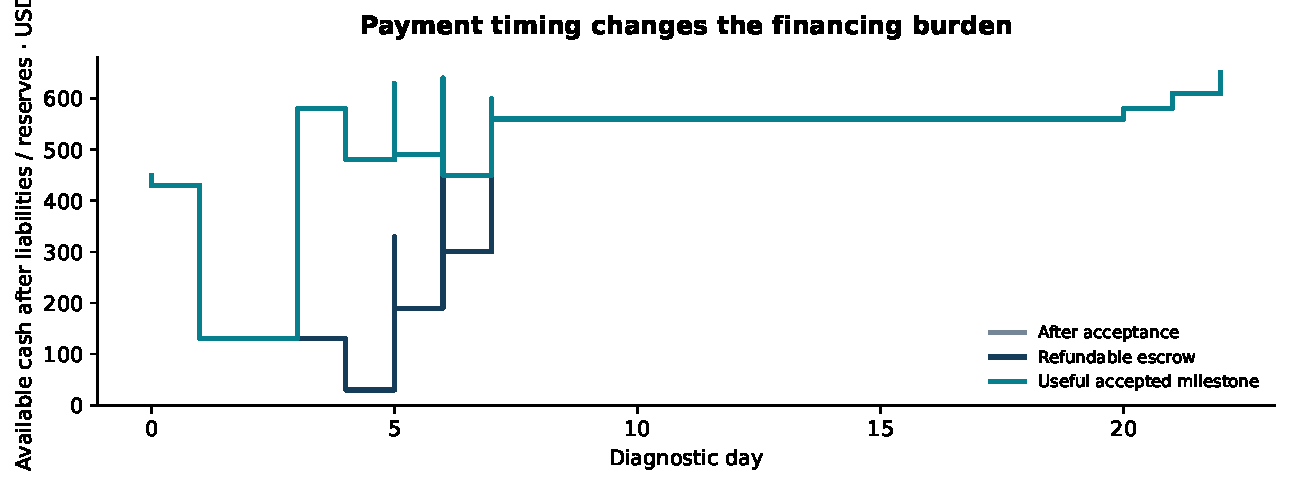
\includegraphics[width=0.97\linewidth]{figures/cash_timing.pdf}\caption{Arbitrary successful diagnostic paths with USD500 opening cash. Refundable principal remains unavailable. The separately useful accepted milestone requires less opening cash only when released early; all three arrangements need USD840 under the ten-day release delay. Identical successful contribution does not imply identical liquidity.}\end{figure}
